\documentclass[11pt,a4paper]{article}

% ====================================================================
% Packages
% ====================================================================
\usepackage[utf8]{inputenc}
\usepackage[T1]{fontenc}
\usepackage{amsmath,amssymb,amsthm}
\usepackage{mathtools}
\usepackage{hyperref}
\usepackage[margin=1in]{geometry}
\usepackage{enumitem}
\usepackage{booktabs}
\usepackage{listings}
\usepackage{xcolor}
\usepackage{cleveref}
\usepackage{natbib}
\usepackage{mdframed}
\usepackage{tikz}
\usetikzlibrary{arrows.meta,positioning,decorations.pathreplacing}

% ====================================================================
% Theorem environments
% ====================================================================
\theoremstyle{plain}
\newtheorem{theorem}{Theorem}[section]
\newtheorem{lemma}[theorem]{Lemma}
\newtheorem{proposition}[theorem]{Proposition}
\newtheorem{corollary}[theorem]{Corollary}

\theoremstyle{definition}
\newtheorem{definition}[theorem]{Definition}
\newtheorem{remark}[theorem]{Remark}

% ====================================================================
% Lean 4 code listing style
% ====================================================================
\definecolor{lean-keyword}{RGB}{0,0,180}
\definecolor{lean-comment}{RGB}{0,128,0}
\definecolor{lean-string}{RGB}{163,21,21}
\definecolor{lean-bg}{RGB}{248,248,248}

\lstdefinelanguage{lean4}{
  keywords={theorem,lemma,def,class,instance,import,open,variable,
            noncomputable,section,namespace,end,where,let,have,show,
            intro,obtain,use,exact,rw,simp,apply,by,fun,match,if,
            then,else,do,return,axiom,abbrev,private,attribute,
            suffices,change,congr,ext,constructor,rintro,push_neg,
            linarith,absurd,set_option,omit,in,set,cases,refine,
            calc,filter_upwards,with,specialize},
  sensitive=true,
  morecomment=[l]{--},
  morecomment=[s]{/-}{-/},
  morestring=[b]",
  morestring=[b]',
}

\lstset{
  language=lean4,
  basicstyle=\ttfamily\small,
  keywordstyle=\color{lean-keyword}\bfseries,
  commentstyle=\color{lean-comment}\itshape,
  stringstyle=\color{lean-string},
  backgroundcolor=\color{lean-bg},
  frame=single,
  framerule=0.5pt,
  breaklines=true,
  breakatwhitespace=true,
  tabsize=2,
  showstringspaces=false,
  numbers=left,
  numberstyle=\tiny\color{gray},
  numbersep=5pt,
  xleftmargin=15pt,
  captionpos=b,
}

% ====================================================================
% Macros
% ====================================================================
\newcommand{\NN}{\mathbb{N}}
\newcommand{\ZZ}{\mathbb{Z}}
\newcommand{\RR}{\mathbb{R}}
\newcommand{\BISH}{\mathrm{BISH}}
\newcommand{\CRM}{\mathrm{CRM}}
\newcommand{\LPO}{\mathrm{LPO}}
\newcommand{\WLPO}{\mathrm{WLPO}}
\newcommand{\LLPO}{\mathrm{LLPO}}
\newcommand{\MP}{\mathrm{MP}}
\newcommand{\FT}{\mathrm{FT}}
\newcommand{\PA}{\mathrm{PA}}
\newcommand{\Lean}{\textsc{Lean~4}}
\newcommand{\Mathlib}{\textsc{Mathlib4}}
\newcommand{\leanok}{\textsf{\small \textcolor{green!70!black}{\checkmark}}}
\newcommand{\norm}[1]{\left\lVert #1 \right\rVert}
\newcommand{\czero}{c_0}
\newcommand{\linf}{\ell^\infty}
\newcommand{\quotgap}{\linf/\czero}

% ====================================================================
% Title
% ====================================================================
\title{%
  \textbf{An Arithmetic Proof That Bidual Gap Detection Is WLPO-Complete}\\[6pt]
  {\normalsize G\"odel Sequences, Explicit Reductions, and a Lean~4 Formalization}%
}

\author{
  Paul Chun-Kit Lee\thanks{%
    New York University.
    AI-assisted formalization; see \S\ref{sec:ai} for methodology.} \\
  New York University \\
  \texttt{dr.paul.c.lee@gmail.com}
}

\date{February 2026}

% ====================================================================
\begin{document}
\maketitle

% ====================================================================
\begin{abstract}
We give a new proof that deciding membership in the bidual gap $\quotgap$
is $\WLPO$-complete over Bishop-style constructive mathematics, independent
of the functional-analytic proof in Paper~2~\citep{Lee26a}. The proof
proceeds via arithmetic: we construct an injective, order-preserving map
$\Phi$ from the Lindenbaum algebra of $\Pi^0_1$ sentences of Peano
Arithmetic into $\quotgap$, using bounded proof-search sequences
(\emph{G\"odel sequences}). We prove that $\Phi([\varphi]) = [0]$ if
and only if $\varphi$ is $\PA$-refutable. Since $\Pi^0_1$ consistency
decidability is known to be $\WLPO$-equivalent, this yields that gap
detection is $\WLPO$-complete by a route entirely independent of
Paper~2. That two unrelated methods---functional-analytic (Paper~2)
and arithmetic (this paper)---both establish $\WLPO$-completeness of
gap detection is evidence that this classification is robust.

The construction is formalized in \Lean{} (1{,}213 lines, 30~standard
axioms for $\PA$ metamathematics, \Mathlib{}-compatible).
\end{abstract}

\tableofcontents

% ====================================================================
\section{Introduction}\label{sec:intro}
% ====================================================================

% --- Paragraph 1: Paper 2's result ---
Paper~2 of this series~\citep{Lee26a} proved that detecting the bidual
gap---deciding whether the canonical embedding $J_X : X \to X^{**}$ is
surjective---is $\WLPO$-complete over $\BISH$. The proof used functional
analysis: an Ishihara kernel extracted from a gap witness, reducing gap
detection to tail-behavior decidability. This established gap detection as
a constructive complexity benchmark.

% --- Paragraph 2: The question ---
Is Paper~2's result an artifact of its proof method, or is the
$\WLPO$-completeness of gap detection a robust classification? An
independent proof via different methods would provide evidence for
robustness.

% --- Paragraph 3: This paper's contribution ---
We prove gap detection is $\WLPO$-complete by an entirely different
route---through arithmetic rather than functional analysis. The proof
constructs an explicit reduction from $\Pi^0_1$ consistency (a known
$\WLPO$-complete problem) to gap membership. Each $\Pi^0_1$
sentence~$\varphi$ maps to a \emph{G\"odel sequence} $v^\varphi$ in $\linf$,
constructed from bounded proof search. The sequence lies in $\czero$ if and
only if $\varphi$ is refutable. The map is injective on $\PA$-equivalence
classes. This reduces $\Pi^0_1$ consistency to gap membership, and since
$\Pi^0_1$ consistency is $\WLPO$-complete (Ishihara~\citep{Ish06};
Bridges--Richman), gap detection is $\WLPO$-complete.

% --- Paragraph 4: Independence ---
This proof shares no machinery with Paper~2. Paper~2 works with dual
spaces, functionals, and thresholds. This paper works with G\"odel
numbering, proof predicates, and sentence equivalence. The two proofs
arrive at the same classification via independent constructions,
confirming that $\WLPO$-completeness of gap detection is not an artifact
of either approach.

% --- Paragraph 5: Scope and limitations ---
The reduction maps into $\quotgap$, which is a mathematical abstraction.
The G\"odel sequences are engineered from the proof predicate. The paper
establishes a complexity-class result, not a physical correspondence.
Physical interpretations of $\WLPO$ are treated in other papers of the
series.

\subsection{Contributions}

\begin{enumerate}
  \item \textbf{G\"odel sequence reduction.} A well-defined injection $\Phi$ from
        the Lindenbaum algebra $\Pi^0_1/{\sim_\PA}$ into $\quotgap$
        (Theorem~\ref{thm:correspondence}).
  \item \textbf{Gap detection theorem.} $\Phi([\varphi]) = [0]$ iff $\varphi$
        is refutable (Theorem~\ref{thm:detection}).
  \item \textbf{Calibration chain.} $\WLPO \iff$ $\Pi^0_1$ consistency
        decidable $\iff$ gap detection decidable
        (Theorem~\ref{thm:calibration}).
  \item \textbf{Machine-checked formalization.} 1{,}213 lines of \Lean{},
        7~modules, built on \Mathlib{}.
\end{enumerate}

% ====================================================================
\section{Arithmetic Side: Axiomatized PA}\label{sec:arithmetic}
% ====================================================================

We axiomatize the properties of Peano Arithmetic needed for the
construction. These are standard metamathematical facts that would be
theorems given a formalization of G\"odel numbering; axiomatizing them
allows us to focus on the reduction itself.

\begin{definition}[Axiomatized syntax of PA]\label{def:syntax}
We postulate:
\begin{itemize}
  \item A type \texttt{SentencePA} of sentences.
  \item An injective function $\texttt{godelNum} : \texttt{SentencePA} \to \NN$.
  \item A decidable proof predicate $\texttt{PrfPA} : \NN \to
        \texttt{SentencePA} \to \mathrm{Prop}$.
  \item Syntactic operations: negation, conjunction, disjunction, implication.
  \item A bottom element $\bot$ (falsity).
\end{itemize}
\end{definition}

\begin{definition}[Provability and consistency]\label{def:provability}
\begin{align*}
\texttt{ProvablePA}(\psi) &\colonequals \exists\, p,\; \texttt{PrfPA}(p, \psi) \\
\texttt{RefutablePA}(\psi) &\colonequals \texttt{ProvablePA}(\lnot\psi) \\
\texttt{ConsistentPA}(\psi) &\colonequals \lnot\,\texttt{RefutablePA}(\psi)
\end{align*}
We axiomatize that $\PA$ is consistent ($\bot$ is not provable).
\end{definition}

\begin{definition}[$\PA$-provable equivalence]\label{def:paequiv}
$\varphi \sim_\PA \psi$ iff $\PA \vdash (\varphi \to \psi) \land (\psi \to \varphi)$.
This is an equivalence relation that respects all syntactic operations and
preserves consistency.
\end{definition}

\begin{definition}[The Lindenbaum algebra]\label{def:lindenbaum}
The type $\Pi^0_1$ consists of those sentences marked as arithmetically
$\Pi^0_1$ (axiomatized as a predicate \texttt{isPi01} closed under $\land$
and~$\lor$). The \emph{Lindenbaum algebra} is
$\texttt{LindenbaumPi01} \colonequals \Pi^0_1/{\sim_\PA}$,
with partial order $[\varphi] \leq [\psi]$ iff $\PA \vdash \varphi \to \psi$.
\end{definition}

\subsection{Canonical G\"odel Numbers}

Each equivalence class in $\texttt{LindenbaumPi01}$ has a canonical G\"odel
number: the minimum G\"odel number among all sentences in the class.

\begin{definition}[Canonical G\"odel number]\label{def:canonGN}
$\texttt{canonGN}(\varphi) \colonequals \min\{n \mid \exists\, \psi \in \Pi^0_1,\;
\texttt{godelNum}(\psi) = n \land \varphi \sim_\PA \psi\}$.
\end{definition}

\begin{lemma}\label{lem:canonGN-well-defined}
$\texttt{canonGN}$ is well-defined on $\texttt{LindenbaumPi01}$:
if $\varphi \sim_\PA \psi$, then $\texttt{canonGN}(\varphi) = \texttt{canonGN}(\psi)$.
\end{lemma}

\begin{proof}
If $\varphi \sim_\PA \psi$, then for any witness $\chi$ with
$\varphi \sim_\PA \chi$, we have $\psi \sim_\PA \chi$ by transitivity,
and vice versa. So the sets of G\"odel numbers are identical, and
their minima agree.
\end{proof}

% ====================================================================
\section{Analytic Side: The Bidual Gap}\label{sec:analytic}
% ====================================================================

\begin{definition}[Sequence spaces]\label{def:seqspaces}
\begin{itemize}
  \item $\linf$: bounded real sequences
        $\{f : \NN \to \RR \mid \exists\, M,\; \forall\, n,\; |f(n)| \leq M\}$.
  \item $\czero$: sequences converging to $0$.
  \item $\quotgap = \linf/\czero$: the \emph{bidual gap}.
\end{itemize}
Two bounded sequences $f, g$ are \emph{$\czero$-equivalent} if $f - g \to 0$.
\end{definition}

\subsection{Row-Based Structure}

We use the Cantor pairing $\langle n, m \rangle : \NN \to \NN$ to decompose
$\NN$ into infinitely many infinite rows.

\begin{definition}[Rows]\label{def:row}
$\mathrm{row}(n) = \{k \in \NN \mid \pi_1(k) = n\}$.
\end{definition}

\begin{lemma}\label{lem:rows}
Each row is infinite. Distinct rows are disjoint.
\end{lemma}

\begin{definition}[Row characteristic functions]\label{def:rowchar}
$\texttt{rowChar}(n)(k) = \begin{cases} 1 & \text{if } \pi_1(k) = n \\ 0 & \text{otherwise}\end{cases}$.
\end{definition}

\begin{lemma}\label{lem:rowchar-not-null}
$\texttt{rowChar}(n) \notin \czero$ for all $n$ (infinitely many 1s).
\end{lemma}

\begin{lemma}\label{lem:rowchar-not-equiv-zero}
$[\texttt{rowChar}(n)] \neq [0]$ in $\quotgap$ for all~$n$.
\end{lemma}

The \emph{logical gap sublattice} $L \subset \quotgap$ consists of $[0]$
together with $\{[\texttt{rowChar}(n)] \mid n \in \NN\}$.

% ====================================================================
\section{The G\"odel Sequence}\label{sec:godelseq}
% ====================================================================

The G\"odel sequence is the bridge between the arithmetic and analytic sides.

\begin{definition}[G\"odel sequence]\label{def:godelseq}
For a sentence $\varphi$ with G\"odel number $g = \texttt{godelNum}(\varphi)$:
\[
v^\varphi(k) \colonequals
\begin{cases}
1 & \text{if } \pi_1(k) = g \text{ and }
    \forall\, p \leq k,\; \lnot\,\texttt{PrfPA}(p, \lnot\varphi), \\
0 & \text{otherwise}.
\end{cases}
\]
\end{definition}

% ====================================================================
% NEW FIGURE: The Gödel sequence as proof search (for Paper 26, §5)
% Insert after Definition 5.1 (the Gödel sequence definition),
% before Theorem 5.2 (refutable => null).
% ====================================================================

\begin{figure}[ht]
\centering
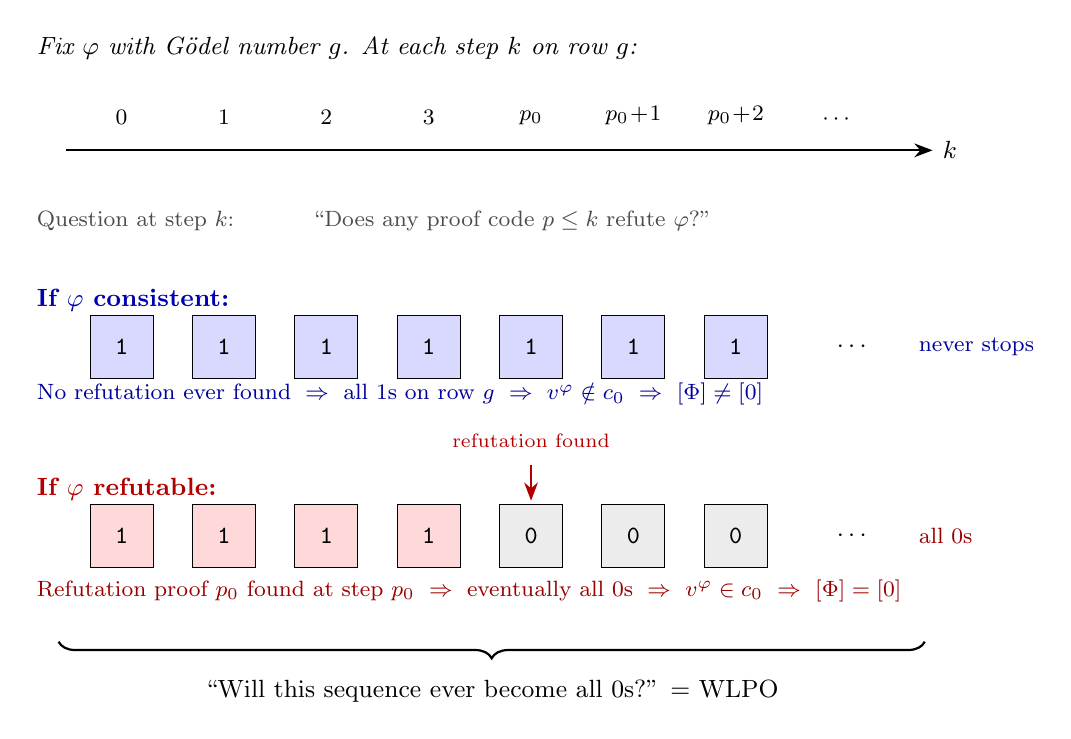
\begin{tikzpicture}[
  >=Stealth,
  seqcell/.style={minimum width=8mm, minimum height=8mm, draw, inner sep=0pt,
               font=\small\ttfamily, anchor=center},
  label/.style={font=\footnotesize, anchor=south},
  timeline/.style={thick, ->},
]

% === Title ===
\node[font=\small\itshape, anchor=west] at (-1.0, 3.8)
  {Fix $\varphi$ with G\"odel number $g$.  At each step $k$ on row $g$:};

% === Timeline arrow ===
\draw[timeline] (-0.5, 2.5) -- (10.5, 2.5) node[right, font=\small] {$k$};

% === Step labels ===
\foreach \x/\lab in {0/0, 1/1, 2/2, 3/3, 4/{p_0}, 5/{p_0\!+\!1}, 6/{p_0\!+\!2}, 7/{\cdots}} {
  \node[label] at (1.3*\x + 0.2, 2.7) {$\lab$};
}

% === Question at each step ===
\node[font=\footnotesize, anchor=west, text=black!70] at (-1.0, 1.6)
  {Question at step $k$:};
\node[font=\footnotesize, anchor=west, text=black!70] at (2.5, 1.6)
  {``Does any proof code $p \leq k$ refute $\varphi$?''};

% === Consistent outcome (top) ===
\node[font=\small\bfseries, text=blue!70!black, anchor=west] at (-1.0, 0.6)
  {If $\varphi$ consistent:};

\foreach \x/\v in {0/1, 1/1, 2/1, 3/1, 4/1, 5/1, 6/1} {
  \node[seqcell, fill=blue!15] at (1.3*\x + 0.2, 0.0) {\v};
}
\node[font=\small] at (9.5, 0.0) {$\cdots$};
\node[font=\footnotesize, anchor=west, text=blue!60!black] at (10.2, 0.0)
  {never stops};

\node[font=\footnotesize, text=blue!60!black, anchor=west] at (-1.0, -0.6)
  {No refutation ever found $\;\Rightarrow\;$ all 1s on row $g$
   $\;\Rightarrow\;$ $v^\varphi \notin c_0$
   $\;\Rightarrow\;$ $[\Phi] \neq [0]$};

% === Refutable outcome (bottom) ===
\node[font=\small\bfseries, text=red!70!black, anchor=west] at (-1.0, -1.8)
  {If $\varphi$ refutable:};

\foreach \x/\v/\col in {0/1/red!15, 1/1/red!15, 2/1/red!15, 3/1/red!15,
                         4/0/gray!15, 5/0/gray!15, 6/0/gray!15} {
  \node[seqcell, fill=\col] at (1.3*\x + 0.2, -2.4) {\v};
}
\node[font=\small] at (9.5, -2.4) {$\cdots$};
\node[font=\footnotesize, anchor=west, text=red!60!black] at (10.2, -2.4)
  {all 0s};

% === Refutation marker ===
\draw[thick, red!70!black, ->] (5.4, -1.5) -- (5.4, -1.95);
\node[font=\scriptsize, text=red!70!black, anchor=south] at (5.4, -1.4)
  {refutation found};

\node[font=\footnotesize, text=red!60!black, anchor=west] at (-1.0, -3.1)
  {Refutation proof $p_0$ found at step $p_0$
   $\;\Rightarrow\;$ eventually all 0s
   $\;\Rightarrow\;$ $v^\varphi \in c_0$
   $\;\Rightarrow\;$ $[\Phi] = [0]$};

% === WLPO annotation ===
\draw[thick, decorate, decoration={brace, amplitude=6pt, mirror, raise=4pt}]
  (-0.6, -3.6) -- (10.4, -3.6);
\node[font=\small, anchor=north] at (4.9, -4.1)
  {``Will this sequence ever become all 0s?''  $=$ WLPO};

\end{tikzpicture}
\caption{The G\"odel sequence as a proof-search process.  At each step $k$,
bounded proof search checks whether any code $p \leq k$ refutes~$\varphi$.
If $\varphi$ is consistent, no refutation is ever found and the sequence
stays at~1 on row~$g$ indefinitely.  If $\varphi$ is refutable, the
sequence drops to~0 once the refutation proof code $p_0$ is reached.
The question ``does this sequence eventually vanish?''\ is precisely
$\WLPO$.}
\label{fig:proof-search}
\end{figure}

The G\"odel sequence is $\{0,1\}$-valued and bounded, hence in $\linf$.

\begin{theorem}[Refutable $\Rightarrow$ null]\label{thm:refutable-null}
If $\varphi$ is refutable, then $v^\varphi$ is eventually zero, hence
$v^\varphi \in \czero$ and $[v^\varphi] = [0]$ in $\quotgap$. \leanok
\end{theorem}

\begin{proof}
If $p_0$ is a proof of $\lnot\varphi$, then for all $k \geq p_0$,
the bounded proof search finds $p_0 \leq k$, so $v^\varphi(k) = 0$.
\end{proof}

\begin{theorem}[Consistent $\Rightarrow$ not null]\label{thm:consistent-not-null}
If $\varphi$ is consistent, then $v^\varphi = \texttt{rowChar}(g)$ pointwise,
hence $v^\varphi \notin \czero$ and $[v^\varphi] \neq [0]$. \leanok
\end{theorem}

\begin{proof}
If $\varphi$ is consistent, no refutation proof exists, so the bounded search
always fails, and $v^\varphi(k) = 1$ whenever $\pi_1(k) = g$. This gives
$v^\varphi = \texttt{rowChar}(g)$ pointwise. Since $\texttt{rowChar}(g)$
has infinitely many 1s, it does not converge to~0.
\end{proof}

% ====================================================================
\section{The G\"odel Sequence Reduction}\label{sec:correspondence}
% ====================================================================

\begin{figure}[ht]
\centering
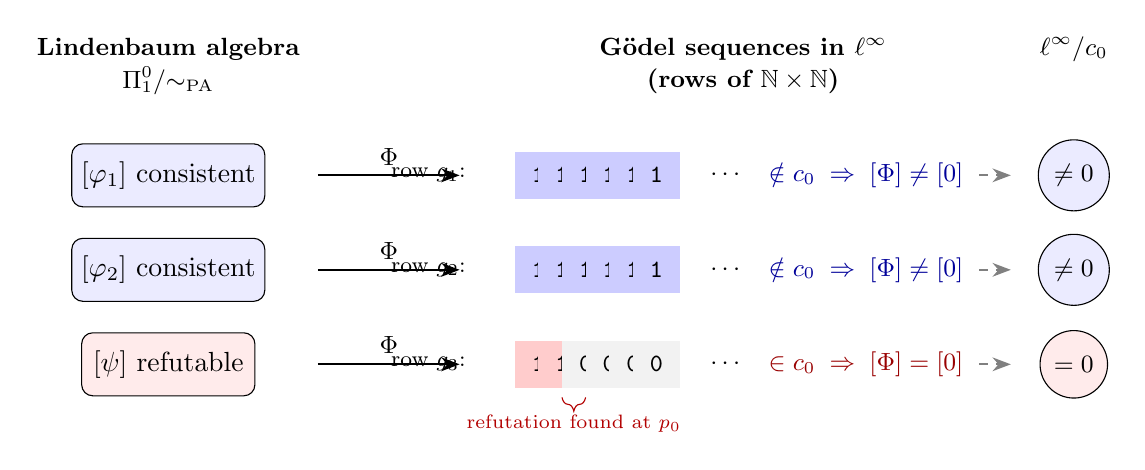
\begin{tikzpicture}[
  >=Stealth,
  row label/.style={anchor=east, font=\small},
  cell/.style={minimum width=6mm, minimum height=6mm, inner sep=0pt,
               font=\small\ttfamily},
  brace/.style={decorate, decoration={brace, amplitude=5pt, raise=2pt}},
]

% === Left side: Lindenbaum algebra ===
\node[font=\bfseries\small] at (-4.5, 3.2) {Lindenbaum algebra};
\node[font=\bfseries\small] at (-4.5, 2.8) {$\Pi^0_1/{\sim_\PA}$};

\node[draw, rounded corners, minimum width=22mm, minimum height=8mm,
      fill=blue!8] (class1) at (-4.5, 1.6) {$[\varphi_1]$ consistent};
\node[draw, rounded corners, minimum width=22mm, minimum height=8mm,
      fill=blue!8] (class2) at (-4.5, 0.4) {$[\varphi_2]$ consistent};
\node[draw, rounded corners, minimum width=22mm, minimum height=8mm,
      fill=red!8] (class3) at (-4.5, -0.8) {$[\psi]$ refutable};

% === Arrow Phi ===
\draw[->, thick, font=\small] (-2.6, 1.6) -- node[above] {$\Phi$} (-0.8, 1.6);
\draw[->, thick, font=\small] (-2.6, 0.4) -- node[above] {$\Phi$} (-0.8, 0.4);
\draw[->, thick, font=\small] (-2.6, -0.8) -- node[above] {$\Phi$} (-0.8, -0.8);

% === Right side: rows of N x N ===
\node[font=\bfseries\small] at (2.8, 3.2) {G\"odel sequences in $\linf$};
\node[font=\bfseries\small] at (2.8, 2.8) {(rows of $\NN \times \NN$)};

% Row g1: consistent -- all 1s on row
\node[row label] at (-0.6, 1.6) {\footnotesize row $g_1$:};
\foreach \x/\v in {0/1,1/1,2/1,3/1,4/1,5/1} {
  \node[cell, fill=blue!20] at (0.3*\x + 0.2, 1.6) {\v};
}
\node[font=\small] at (2.6, 1.6) {$\cdots$};
\node[font=\small, anchor=west, text=blue!60!black] at (3.0, 1.6)
  {$\notin \czero \;\Rightarrow\; [\Phi] \neq [0]$};

% Row g2: consistent -- all 1s on row
\node[row label] at (-0.6, 0.4) {\footnotesize row $g_2$:};
\foreach \x/\v in {0/1,1/1,2/1,3/1,4/1,5/1} {
  \node[cell, fill=blue!20] at (0.3*\x + 0.2, 0.4) {\v};
}
\node[font=\small] at (2.6, 0.4) {$\cdots$};
\node[font=\small, anchor=west, text=blue!60!black] at (3.0, 0.4)
  {$\notin \czero \;\Rightarrow\; [\Phi] \neq [0]$};

% Row g3: refutable -- 1s then 0s after refutation
\node[row label] at (-0.6, -0.8) {\footnotesize row $g_3$:};
\foreach \x/\v in {0/1,1/1,2/0,3/0,4/0,5/0} {
  \pgfmathparse{\v > 0 ? "red!20" : "gray!10"}
  \edef\fillcol{\pgfmathresult}
  \node[cell, fill=\fillcol] at (0.3*\x + 0.2, -0.8) {\v};
}
\node[font=\small] at (2.6, -0.8) {$\cdots$};
\node[font=\small, anchor=west, text=red!60!black] at (3.0, -0.8)
  {$\in \czero \;\Rightarrow\; [\Phi] = [0]$};

% Refutation marker
\draw[brace, red!70!black] (0.8, -1.15) -- node[below=5pt, font=\scriptsize,
  text=red!70!black] {refutation found at $p_0$} (0.5, -1.15);

% === Far right: gap quotient ===
\node[font=\bfseries\small] at (7.0, 3.2) {$\quotgap$};

\draw[->, thick, dashed, gray] (5.8, 1.6) -- (6.2, 1.6);
\draw[->, thick, dashed, gray] (5.8, 0.4) -- (6.2, 0.4);
\draw[->, thick, dashed, gray] (5.8, -0.8) -- (6.2, -0.8);

\node[draw, circle, minimum size=8mm, fill=blue!8,
      font=\small] at (7.0, 1.6) {$\neq 0$};
\node[draw, circle, minimum size=8mm, fill=blue!8,
      font=\small] at (7.0, 0.4) {$\neq 0$};
\node[draw, circle, minimum size=8mm, fill=red!8,
      font=\small] at (7.0, -0.8) {$= 0$};

\end{tikzpicture}
\caption{The G\"odel sequence reduction map $\Phi$. Each equivalence class $[\varphi]$
in the Lindenbaum algebra occupies a unique row of $\NN \times \NN$.
Consistent sentences produce constant-1 rows (not in $\czero$, hence
nonzero in $\quotgap$). Refutable sentences collapse to 0 once a
refutation proof is found (eventually zero, hence in $\czero$, mapping
to $[0]$ in $\quotgap$).}
\label{fig:godelgap}
\end{figure}

\subsection{Canonical Representatives}

For each equivalence class in $\texttt{LindenbaumPi01}$, we select the
\emph{canonical representative}: the $\Pi^0_1$ sentence with the smallest
G\"odel number in the class. This is well-defined by the well-ordering
of~$\NN$ and uses \texttt{Nat.find} with classical decidability.

\begin{definition}[G\"odel sequence reduction map]\label{def:godelgapmap}
$\Phi : \texttt{LindenbaumPi01} \to \quotgap$ sends each class $[\varphi]$
to $[v^{\texttt{canonRep}(\varphi)}]$, the gap element of the canonical
representative's G\"odel sequence.
\end{definition}

\begin{lemma}[Well-definedness]\label{lem:well-defined}
$\Phi$ is well-defined: if $\varphi \sim_\PA \psi$, then
$\texttt{canonRep}(\varphi) = \texttt{canonRep}(\psi)$ (they have the same
canonical G\"odel number, and $\texttt{godelNum}$ is injective), so
their G\"odel sequences are identical. \leanok
\end{lemma}

\begin{theorem}[Injectivity]\label{thm:injectivity}
$\Phi$ is injective.
\end{theorem}

\begin{proof}
Suppose $\Phi([\varphi]) = \Phi([\psi])$. Four cases:
\begin{enumerate}
  \item \emph{Both consistent:} their G\"odel sequences agree with
        $\texttt{rowChar}(g_\varphi)$ and $\texttt{rowChar}(g_\psi)$
        respectively. If the gap elements are equal, the row characteristic
        functions are $\czero$-equivalent, forcing $g_\varphi = g_\psi$
        (different rows give non-equivalent indicators). Since
        $\texttt{godelNum}$ is injective, the canonical representatives
        are identical, so $[\varphi] = [\psi]$.
  \item \emph{$\varphi$ consistent, $\psi$ refutable:} $\Phi([\varphi]) \neq [0]$
        but $\Phi([\psi]) = [0]$, contradiction. \leanok
  \item \emph{$\varphi$ refutable, $\psi$ consistent:} symmetric. \leanok
  \item \emph{Both refutable:} both are $\PA$-equivalent to $\bot$, hence
        to each other, so $[\varphi] = [\psi]$. \leanok
\end{enumerate}
\end{proof}

\begin{theorem}[G\"odel Sequence Reduction]\label{thm:correspondence}
The map $\Phi : \texttt{LindenbaumPi01} \to \quotgap$ is injective,
maps refutable classes to $[0]$, and maps consistent classes to nonzero
elements of~$\quotgap$. \leanok
\end{theorem}

\begin{theorem}[Gap Detection]\label{thm:detection}
$\Phi([\varphi]) = [0]$ if and only if $\varphi$ is refutable over $\PA$. \leanok
\end{theorem}

% ====================================================================
\section{Calibration Link}\label{sec:calibration}
% ====================================================================

We connect the G\"odel sequence reduction to the omniscience hierarchy.

\begin{definition}[$\Pi^0_1$ consistency decidability]\label{def:pi01-decidable}
$\text{$\Pi^0_1$ consistency decidable}$ iff for every $\Pi^0_1$
sentence~$\varphi$, either $\varphi$ is consistent or $\varphi$ is refutable.
\end{definition}

\begin{definition}[Gap detection decidability]\label{def:gap-decidable}
Gap detection is decidable iff for every $\Pi^0_1$ sentence~$\varphi$,
either $\Phi([\varphi]) = [0]$ or $\Phi([\varphi]) \neq [0]$.
\end{definition}

\begin{theorem}[$\WLPO \Rightarrow \Pi^0_1$ consistency decidable]\label{thm:wlpo-forward}
$\WLPO$ implies $\Pi^0_1$ consistency is decidable. \leanok
\end{theorem}

\begin{proof}
Given $\WLPO$ and a $\Pi^0_1$ sentence $\varphi$, define the binary
sequence $\alpha(n) = 1$ if $\exists\, p \leq n,\; \texttt{PrfPA}(p, \lnot\varphi)$,
else $\alpha(n) = 0$. Then $(\forall n.\; \alpha(n) = 0) \iff \texttt{ConsistentPA}(\varphi)$.
$\WLPO$ decides whether $\alpha$ is identically zero.
\end{proof}

\begin{theorem}[Calibration chain]\label{thm:calibration}
\[
\WLPO \iff \text{$\Pi^0_1$ consistency decidable}
       \iff \text{gap detection decidable}. \quad \leanok
\]
\end{theorem}

\begin{proof}
The first equivalence is $\WLPO \Rightarrow$ (Theorem~\ref{thm:wlpo-forward})
and the reverse (axiomatized: given a binary sequence $\alpha$, construct
the $\Pi^0_1$ sentence ``$\forall n.\; \alpha(n) = 0$'' and decide its
consistency). The second equivalence follows directly from the gap detection
theorem (Theorem~\ref{thm:detection}).
\end{proof}

% ====================================================================
\section{Formalization}\label{sec:formalization}
% ====================================================================

\subsection{Module Structure}

\begin{table}[h]
\centering
\begin{tabular}{llr}
\toprule
\textbf{Module} & \textbf{Content} & \textbf{Lines} \\
\midrule
\texttt{Basic.lean} & WLPO, $\linf$, $\czero$, $\quotgap$ & 110 \\
\texttt{ArithmeticSide.lean} & Axiomatized PA, Lindenbaum algebra & 291 \\
\texttt{AnalyticSide.lean} & Rows, $\texttt{rowChar}$, logical gap sublattice & 131 \\
\texttt{GodelSequence.lean} & G\"odel sequence $v^\varphi$, key properties & 147 \\
\texttt{Correspondence.lean} & $\Phi$, injectivity, gap detection & 220 \\
\texttt{CalibrationLink.lean} & $\WLPO \iff$ gap detection & 137 \\
\texttt{Main.lean} & Aggregator and axiom audit & 177 \\
\midrule
\textbf{Total} & & \textbf{1{,}213} \\
\bottomrule
\end{tabular}
\caption{Module structure of the \Lean{} formalization.}
\label{tab:modules}
\end{table}

\subsection{Axiom Profile}

The formalization uses 30~custom axioms, all encoding standard
metamathematical facts about $\PA$:

\begin{itemize}
  \item \textbf{Type axioms (4):} \texttt{SentencePA}, \texttt{godelNum},
        \texttt{PrfPA}, \texttt{botPA}.
  \item \textbf{Function axioms (4):} \texttt{negPA}, \texttt{andPA},
        \texttt{orPA}, \texttt{implPA}.
  \item \textbf{Decidability (2):} \texttt{PrfPA\_decidable},
        \texttt{bounded\_refutation\_decidable}.
  \item \textbf{Structural (2):} \texttt{godelNum\_injective},
        \texttt{pa\_consistent}.
  \item \textbf{$\Pi^0_1$ (4):} \texttt{isPi01}, \texttt{pi01\_bot},
        \texttt{pi01\_and}, \texttt{pi01\_or}.
  \item \textbf{PAEquiv (7):} reflexivity, symmetry, transitivity,
        consistency preservation, and congruences for $\lnot$, $\land$, $\lor$.
  \item \textbf{PAImplies (4):} reflexivity, transitivity,
        equivalence-to-mutual-implication, congruence.
  \item \textbf{Refutability (1):} \texttt{refutable\_equiv\_bot}.
  \item \textbf{Order preservation (1):}
        \texttt{paImplies\_preserves\_consistency}.
  \item \textbf{Calibration (1):} \texttt{pi01\_decidable\_implies\_wlpo}.
\end{itemize}

All custom axioms would be theorems given a formalization of G\"odel numbering.
The construction works for any consistent, recursively axiomatized theory.

\begin{remark}\label{rem:representability}
The axiom \texttt{pi01\_decidable\_implies\_wlpo} encodes the reverse
direction of the calibration: given a binary sequence $\alpha$, construct
the $\Pi^0_1$ sentence ``$\forall n.\; \alpha(n) = 0$.'' This requires
that primitive recursive predicates are representable in $\PA$---a
standard result (G\"odel, 1931, \S\S5--6) but one that goes beyond the
scope of this formalization.
\end{remark}

\subsection{Sorries}

Three technical sorries remain:
\begin{enumerate}
  \item \texttt{classGN\_injective}: different equivalence classes have
        different canonical G\"odel numbers. (Requires showing the
        \texttt{Nat.find} witnesses for the two classes agree.)
  \item \texttt{rowChar\_neq\_mod\_c0}: characteristic functions of
        different rows are not $\czero$-equivalent. (The difference is $\pm 1$
        on two disjoint infinite sets.)
  \item \texttt{godelGapMap\_injective} (both-consistent case): uses
        sorry~2 above.
\end{enumerate}
These are all mathematically straightforward; the first two are essentially
facts about well-orderings and indicator functions of disjoint infinite sets.

\subsection{Standard Lean Axioms}

The standard \Lean{} axioms \texttt{propext}, \texttt{Classical.choice}, and
\texttt{Quot.sound} appear throughout. \texttt{Classical.choice} enters via
quotient operations, \texttt{Nat.find}, and \Mathlib{}'s filter/metric
infrastructure. This is consistent with the project's use of classical
metatheory.

% ====================================================================
\section{CRM Calibration Summary}\label{sec:crm}
% ====================================================================

\begin{table}[h]
\centering
\begin{tabular}{llll}
\toprule
\textbf{Result} & \textbf{Principle} & \textbf{Status} & \textbf{Paper} \\
\midrule
Bidual gap $\neq 0$ & $\WLPO$ & Calibrated & 2 \\
Gap detection decidable & $\WLPO$ & Calibrated & 26 \\
$\Pi^0_1$ consistency decidable & $\WLPO$ & Calibrated & 26 \\
$\Pi^0_1/{\sim_\PA}$ embeds into $\quotgap$ & (structural) & Verified & 26 \\
\bottomrule
\end{tabular}
\caption{CRM calibration results for the bidual gap and arithmetic consistency.}
\label{tab:calibration}
\end{table}

Gap detection is $\WLPO$-complete, independently confirmed by two
unrelated proofs (functional-analytic in Paper~2, arithmetic in this
paper). The logical cost of detecting the bidual gap is exactly the cost
of deciding $\Pi^0_1$ consistency.

% ====================================================================
\section{Independence, Robustness, and the Constructive Complexity Classification}\label{sec:discussion}
% ====================================================================

% ====================================================================
% FIGURE 3: From physical question to complexity classification
% All three examples calibrate at WLPO (not LPO).
% Papers 2 (gap detection), 7 (singular states), 20 (phase classification).
% ====================================================================

\begin{figure}[ht]
\centering
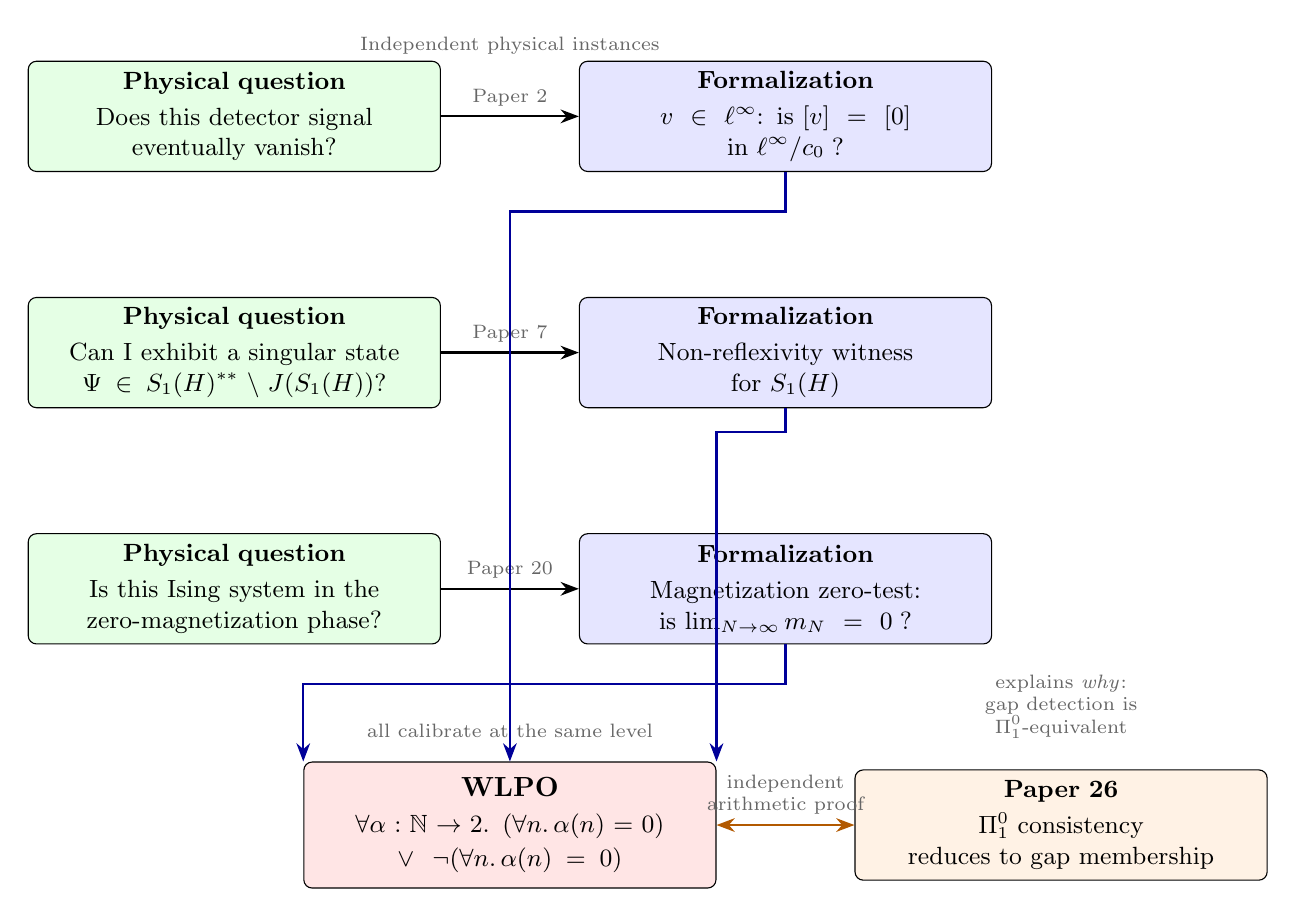
\begin{tikzpicture}[
  >=Stealth,
  box/.style={draw, rounded corners=3pt, minimum width=52mm,
              minimum height=14mm, align=center, font=\small,
              text width=50mm},
  arrow/.style={->, thick, font=\footnotesize},
  annot/.style={font=\scriptsize, text=black!60, align=center},
]

% === Column 1: Physical questions ===
\node[box, fill=green!10] (phys1) at (0, 4.5)
  {\textbf{Physical question}\\[2pt]
   Does this detector signal\\eventually vanish?};

\node[box, fill=green!10] (phys2) at (0, 1.5)
  {\textbf{Physical question}\\[2pt]
   Can I exhibit a singular state\\
   $\Psi \in S_1(H)^{**} \setminus J(S_1(H))$?};

\node[box, fill=green!10] (phys3) at (0, -1.5)
  {\textbf{Physical question}\\[2pt]
   Is this Ising system in the\\
   zero-magnetization phase?};

% === Column 2: Mathematical formalization ===
\node[box, fill=blue!10] (math1) at (7, 4.5)
  {\textbf{Formalization}\\[2pt]
   $v \in \ell^\infty$: is $[v] = [0]$\\
   in $\ell^\infty/c_0$\;?};

\node[box, fill=blue!10] (math2) at (7, 1.5)
  {\textbf{Formalization}\\[2pt]
   Non-reflexivity witness\\
   for $S_1(H)$};

\node[box, fill=blue!10] (math3) at (7, -1.5)
  {\textbf{Formalization}\\[2pt]
   Magnetization zero-test:\\
   is $\lim_{N \to \infty} m_N = 0$\;?};

% === Arrows from physical to formal ===
\draw[arrow] (phys1) -- (math1) node[midway, above, annot] {Paper 2};
\draw[arrow] (phys2) -- (math2) node[midway, above, annot] {Paper 7};
\draw[arrow] (phys3) -- (math3) node[midway, above, annot] {Paper 20};

% === Convergence to WLPO ===
\node[box, fill=red!10, minimum width=45mm, minimum height=16mm,
      font=\normalsize] (wlpo) at (3.5, -4.5)
  {\textbf{WLPO}\\[2pt]
   \small $\forall \alpha\!:\!\mathbb{N}\!\to\!2.\;
   (\forall n.\,\alpha(n)\!=\!0)$\\
   $\lor\;\lnot(\forall n.\,\alpha(n)\!=\!0)$};

\draw[arrow, blue!60!black] (math1.south) -- ++(0,-0.5) -| (wlpo.north);
\draw[arrow, blue!60!black] (math2.south) -- ++(0,-0.3) -| (wlpo.north east);
\draw[arrow, blue!60!black] (math3.south) -- ++(0,-0.5) -| (wlpo.north west);

% === Paper 26's contribution ===
\node[box, fill=orange!10, minimum width=45mm] (p26) at (10.5, -4.5)
  {\textbf{Paper 26}\\[2pt]
   \small $\Pi^0_1$ consistency\\
   reduces to gap membership};

\draw[arrow, orange!70!black, <->] (wlpo) -- node[above, annot]
  {independent\\arithmetic proof} (p26);

% === Annotations ===
\node[annot] at (3.5, 5.4) {Independent physical instances};
\node[annot] at (3.5, -3.3) {all calibrate at the same level};
\node[annot, text width=30mm] at (10.5, -3.0)
  {explains \emph{why}:\\
   gap detection is\\
   $\Pi^0_1$-equivalent};

\end{tikzpicture}
\caption{Multiple independent physical questions (left) formalize as
mathematical problems (right) that all calibrate at $\WLPO$.
Paper~26 provides an arithmetic explanation: gap detection is
$\WLPO$-complete because $\ell^\infty/c_0$ admits a reduction
from $\Pi^0_1$ consistency.  The physical questions are real;
the bidual gap is the mathematical obstruction that explains
their shared logical cost; Paper~26's reduction explains
why this obstruction sits at the $\Pi^0_1$ level of the
arithmetic hierarchy.}
\label{fig:physical-chain}
\end{figure}

\subsection{Two Proofs, One Result}

Paper~2 and this paper independently prove that gap detection is
$\WLPO$-complete. Paper~2's proof is functional-analytic: it extracts
an Ishihara kernel from a gap witness. This paper's proof is arithmetic:
it reduces $\Pi^0_1$ consistency to gap membership via G\"odel sequences.
The methods share no common machinery. The shared conclusion is therefore
robust---$\WLPO$-completeness of gap detection is not an artifact of
either proof technique.

\subsection{Why Two Proofs Matter}

In complexity theory, a single proof that a problem is NP-complete might
depend on features of the specific reduction. Multiple independent
reductions from different NP-complete problems provide stronger evidence
that the classification is natural. Similarly, two independent proofs
of $\WLPO$-completeness from different mathematical domains (functional
analysis and arithmetic) provide stronger evidence that gap detection is
genuinely $\WLPO$-complete, not just ``provably equivalent to $\WLPO$
by a clever trick.''

\subsection{The Reduction as Complexity-Class Identification}

The G\"odel sequence construction reduces $\Pi^0_1$ consistency to gap
membership. Combined with the known $\WLPO \iff \Pi^0_1$ equivalence,
this places gap detection in the $\Pi^0_1$ decidability class. Every
$\WLPO$-calibrated problem in the CRM programme (bidual gap, singular
state witnessing, phase classification, etc.)\ is therefore
$\Pi^0_1$-equivalent---it is exactly
as hard as deciding consistency of arithmetic sentences. This gives
the $\WLPO$ level of the calibration table an arithmetic characterization.

\subsection{Relation to Cubitt et al.}

Cubitt--Perez-Garcia--Wolf reduced the halting problem
($\Sigma^0_1$-complete) to spectral gap existence. That sits above $\LPO$
in the constructive hierarchy. This paper reduces $\Pi^0_1$ consistency
($\WLPO$-complete) to gap membership in $\quotgap$. Both are reduction
results placing analytic problems in arithmetic complexity classes, at
different levels of the hierarchy.

\subsection{Limitations}

\begin{enumerate}
  \item $\quotgap$ is not physical---it is a mathematical abstraction.
  \item The G\"odel sequences are engineered from the proof predicate.
  \item The paper establishes a complexity-class result, not a physical result.
  \item The order-embedding is not a lattice isomorphism---honestly
        downgraded from earlier claims.
  \item The 30~$\PA$ metamathematics axioms are standard but would require
        significant formalization effort to eliminate.
\end{enumerate}

\subsection{What the Two Proofs Together Suggest}

Paper~2 showed that gap detection is hard for functional-analytic
reasons (dual space structure forces $\WLPO$). This paper shows that
gap detection is hard for arithmetic reasons ($\Pi^0_1$ sentences embed
into the gap). That both routes yield $\WLPO$ suggests that
$\WLPO$-completeness captures something intrinsic about the gap, not
something imposed by a particular proof strategy. Whether this intrinsic
character can be made precise (e.g., via a completeness theorem for
$\WLPO$ reductions) is an open question.

% ====================================================================
\section{AI-Assisted Methodology}\label{sec:ai}
% ====================================================================

The formalization was developed with AI assistance (Claude, Anthropic).
The division of labor:
\begin{itemize}
  \item \textbf{Human:} mathematical conception, proof strategy, axiom design,
        verification of correctness.
  \item \textbf{AI:} \Lean{} code generation, debugging, iterative build-fix cycles.
\end{itemize}
All mathematical content was designed by the human author.
The AI served as a programming assistant for the \Lean{} implementation.

% ====================================================================
\section{Conclusion}\label{sec:conclusion}
% ====================================================================

We have given an arithmetic proof, independent of Paper~2~\citep{Lee26a},
that bidual gap detection is $\WLPO$-complete, via explicit reduction from
$\Pi^0_1$ consistency through G\"odel sequences, formalized in \Lean{}.

The G\"odel sequence construction embeds the Lindenbaum algebra of
$\Pi^0_1$ sentences into $\quotgap$, with $\Phi([\varphi]) = [0]$
if and only if $\varphi$ is refutable. Combined with the known
$\WLPO \iff \Pi^0_1$ equivalence, this yields the calibration chain
$\WLPO \iff \text{$\Pi^0_1$ consistency decidable} \iff
\text{gap detection decidable}$ by a route that shares no machinery
with Paper~2's functional-analytic proof.

That two independent methods---one from functional analysis, one from
arithmetic---both establish $\WLPO$-completeness of gap detection is
evidence that this classification is robust: it captures something
intrinsic about the gap, not something imposed by a particular proof
strategy.

% ====================================================================
\section*{Data Availability}
% ====================================================================

The \Lean{} source code is available at:
\begin{center}
\url{https://doi.org/10.5281/zenodo.XXXXXXX}
\end{center}
Verified with \texttt{leanprover/lean4:v4.28.0-rc1} and current \Mathlib{}.

% ====================================================================
\appendix
\section{Selected Lean Code}\label{sec:appendix}
% ====================================================================

\subsection{The G\"odel Sequence}

\begin{lstlisting}[caption={The G\"odel sequence (GodelSequence.lean).}]
noncomputable def godelSeq (phi : SentencePA) : N -> R :=
  fun k =>
    if k.unpair.1 = godelNum phi &&
       forall p, p <= k -> not (PrfPA p (negPA phi))
    then 1
    else 0
\end{lstlisting}

\subsection{Refutable Implies Null}

\begin{lstlisting}[caption={Refutable sentences produce null sequences (GodelSequence.lean).}]
theorem godelSeq_refutable_eventually_zero (phi : SentencePA)
    (href : RefutablePA phi) :
    exists N, forall k >= N, godelSeq phi k = 0 := by
  obtain <<p0, hp0>> := href
  exact <<p0, fun k hk => by
    simp only [godelSeq]
    rw [if_neg]
    push_neg
    intro _hrow
    exact <<p0, hk, hp0>>>>
\end{lstlisting}

\subsection{Gap Detection Theorem}

\begin{lstlisting}[caption={Gap detection (Correspondence.lean).}]
theorem godelGap_detects_refutability (phi : Pi01) :
    godelGapMap (LindenbaumPi01.mk phi) = BidualGap.zero
    <-> RefutablePA phi.val := by
  constructor
  . intro h
    by_contra hcon
    exact godelGapMap_consistent_ne_zero phi hcon h
  . exact godelGapMap_refutable phi
\end{lstlisting}

\subsection{Calibration Chain}

\begin{lstlisting}[caption={WLPO iff gap detection (CalibrationLink.lean).}]
theorem wlpo_iff_gap_detection :
    WLPO <-> GapDetectionDecidable :=
  wlpo_iff_pi01_decidable.trans pi01_decidable_iff_gap_detection
\end{lstlisting}

% ====================================================================
\bibliographystyle{plainnat}

\begin{thebibliography}{20}

\bibitem[Bishop(1967)]{Bis67}
E.~Bishop,
\emph{Foundations of Constructive Analysis},
McGraw-Hill, 1967.

\bibitem[Bishop and Bridges(1985)]{BB85}
E.~Bishop and D.~Bridges,
\emph{Constructive Analysis},
Springer, 1985.

\bibitem[Bridges and V\^{\i}\c{t}\u{a}(2006)]{BV06}
D.~Bridges and L.~V\^{\i}\c{t}\u{a},
\emph{Techniques of Constructive Analysis},
Springer, 2006.

\bibitem[G\"odel(1931)]{God31}
K.~G\"odel,
``\"Uber formal unentscheidbare S\"atze der Principia Mathematica
und verwandter Systeme~I,''
\emph{Monatshefte f\"ur Mathematik und Physik}, 38:173--198, 1931.

\bibitem[Ishihara(2006)]{Ish06}
H.~Ishihara,
``Reverse mathematics in Bishop's constructive mathematics,''
\emph{Philosophia Scientiae}, Cahier sp\'ecial 6:43--59, 2006.

\bibitem[Lee(2026a)]{Lee26a}
P.~C.-K.~Lee,
``The bidual gap of $\ell^\infty/c_0$ as a calibration standard for WLPO,''
2026. Paper~2 in the CRM series.

\bibitem[Lee(2026b)]{Lee26b}
P.~C.-K.~Lee,
``Technical synthesis: logical geography of constructive reverse
mathematics from density matrices to the choice axis,''
2026. Paper~10 in the CRM series (v3.1).

\bibitem[Lee(2026c)]{Lee26c}
P.~C.-K.~Lee,
``Historical synthesis: from Brouwer's bar theorem to the omniscience
hierarchy in mathematical physics,''
2026. Paper~12 in the CRM series.

\bibitem[Lindenbaum(1935)]{Lin35}
A.~Lindenbaum,
``Sur les ensembles ordonn\'es,''
\emph{Comptes Rendus des S\'eances de la Soci\'et\'e des Sciences
et des Lettres de Varsovie}, Classe~III, 28:32--35, 1935.

\bibitem[Simpson(2009)]{Sim09}
S.~Simpson,
\emph{Subsystems of Second Order Arithmetic}, 2nd~ed.,
Cambridge University Press, 2009.

\end{thebibliography}

\end{document}
